% =====================================================================
%  G6 - Cryptographic primitive timing (log scale)
%  --------------------------------------------------------------------
%  Backs claim: Kyber (26 microseconds) negligible vs Paillier (8.69 ms)
%  Source: chapter4.tex Table tab:micro
% =====================================================================
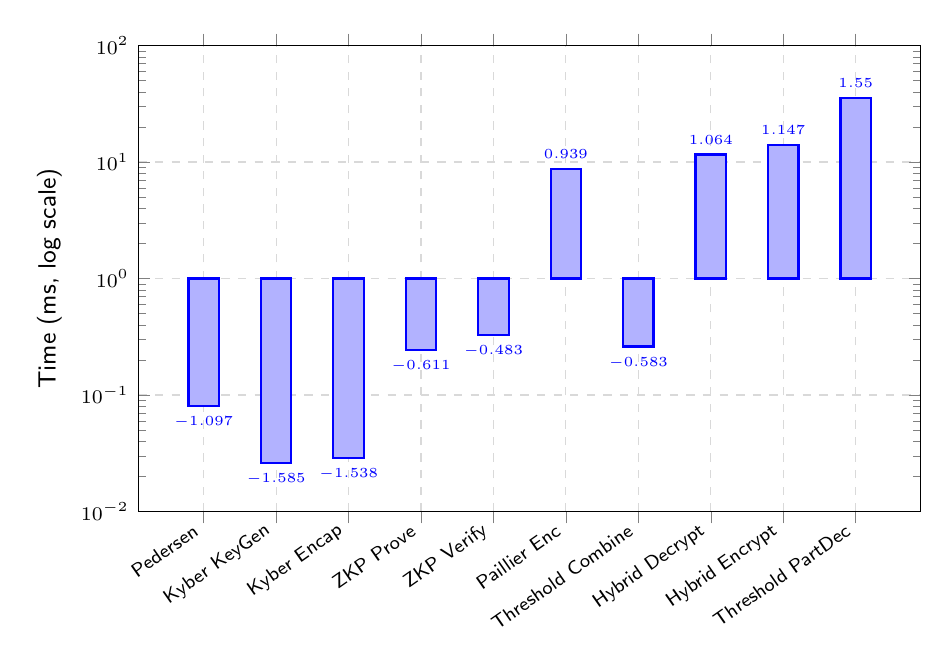
\begin{tikzpicture}
\begin{axis}[
    width=0.95\textwidth,
    height=7.5cm,
    ybar,
    ymode=log,
    log basis y=10,
    ymin=0.01, ymax=100,
    ylabel={Time (ms, log scale)},
    symbolic x coords={
        {Pedersen},
        {Kyber KeyGen},
        {Kyber Encap},
        {ZKP Prove},
        {ZKP Verify},
        {Paillier Enc},
        {Threshold Combine},
        {Hybrid Decrypt},
        {Hybrid Encrypt},
        {Threshold PartDec}
    },
    xtick=data,
    bar width=11pt,
    nodes near coords,
    nodes near coords align={vertical},
    nodes near coords style={font=\sffamily\tiny, /pgf/number format/.cd, fixed, precision=3},
    x tick label style={rotate=35, anchor=east, font=\sffamily\scriptsize},
    grid=major,
    grid style={dashed, gray!30},
    label style={font=\sffamily\small},
    tick label style={font=\sffamily\scriptsize},
    every axis plot/.append style={fill=gray!25, draw=black, thick},
]
\addplot+[ybar] coordinates {
    ({Pedersen},          0.080)
    ({Kyber KeyGen},      0.026)
    ({Kyber Encap},       0.029)
    ({ZKP Prove},         0.245)
    ({ZKP Verify},        0.329)
    ({Paillier Enc},      8.690)
    ({Threshold Combine}, 0.261)
    ({Hybrid Decrypt},   11.600)
    ({Hybrid Encrypt},   14.040)
    ({Threshold PartDec},35.520)
};
\end{axis}
\end{tikzpicture}
